%
% hypkurv.tex -- Hyperbeln und Geraden erzeugen eine Fläche
%
% (c) 2019 Prof Dr Andreas Müller, Hochschule Rapperswil
%
\documentclass[tikz,12pt]{standalone}
\usepackage{amsmath}
\usepackage{times}
\usepackage{txfonts}
\usepackage{color}
\usepackage{pgfplots}
\usepackage{csvsimple}
\usetikzlibrary{arrows,intersections,math}
\begin{document}
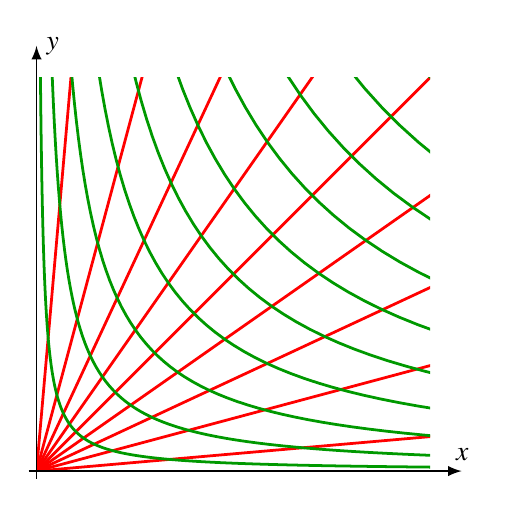
\begin{tikzpicture}[>=latex]

\begin{scope}
\clip (0,0) rectangle (5,5);

\draw[color=red,line width=1pt] (0,0)--(6,6);
\foreach \c in {10,20,...,45}{
	\draw[color=red,line width=1pt] (0,0)--({7*cos(45-\c)},{7*sin(45-\c)});
	\draw[color=red,line width=1pt] (0,0)--({7*cos(45+\c)},{7*sin(45+\c)});
}

\definecolor{darkgreen}{rgb}{0,0.6,0}

\foreach \c in {0.5,1,...,6}{
	\draw[line width=1pt,color=darkgreen]
		plot[domain=-2.5:2.5,samples=100] ({\c*exp(\x)},{\c*exp(-\x)});
}

\end{scope}

\draw[->,line width=0.7pt] (-0.1,0)--(5.4,0) coordinate[label={$x$}];
\draw[->,line width=0.7pt] (0,-0.1)--(0,5.4) coordinate[label={right:$y$}];

\end{tikzpicture}
\end{document}

